\chapter*{付録}
\label{chap:appendix}
\addcontentsline{toc}{chapter}{付録} % 目次に載せる

\setcounter{section}{0} % section の番号をゼロにリセットする
\renewcommand{\thesection}{\Alph{section}} % 数字ではなくアルファベットで数える
\setcounter{equation}{0} % 式番号を A.1 のようにする
\renewcommand{\theequation}{\Alph{section}.\arabic{equation}}
\setcounter{figure}{0} % 図番号
\renewcommand{\thefigure}{\Alph{section}.\arabic{figure}}
\setcounter{table}{0} % 表番号
\renewcommand{\thetable}{\Alph{section}.\arabic{table}}

\section{プログラミング環境の構築}
もし天に限らず、データ解析にはプログラミングが必須となりますが、まず環境がなければ解析を行うことはできません。ひと口にプログラミングと言っても、様々な言語が存在し、それぞれに特色があります。例えばPythonの実行環境にはAnaconda社提供の「Anaconda」\footnote{\url{https://www.anaconda.com/products/individual}}やGoogle社提供の「Google Colaboratory」\footnote{\url{https://colab.research.google.com}}などの有名なものがありますが、ここでは統合開発環境をおすすめしたいと思います。AnacondaやGoogle ColaboratoryはPythonに特化した環境になっていますが、統合開発環境は自分で拡張機能を追加することによって、自分好みのスタイルでPythonだけでなく、C/C++やHTML/CSS、 \LaTeX などの様々な言語を扱うことができるものです。統合開発環境にも同じく様々なものがありますが、その中でも特に有名と言える、Microsoft社提供の「Visual Studio Code」通称「VSCode」\footnote{\url{https://code.visualstudio.com/}}をおすすめします。VSCodeは2015年が最初のリリースと、非常に新しいエディタですが、さすがMicrosoftというべきか、今では非常に多くの人に使われています。個人的にはGithub社提供の「Atom」という統合開発環境が好きでずっと使っていたのですが、Github社がMicrosoft社に買収された影響もあって、2022年の12月で開発終了にまで追い込まれてしまいました。

\subsection{VSCodeのインストール}
まずはインストールしてみましょう。
\begin{figure}[h]
	\centering
	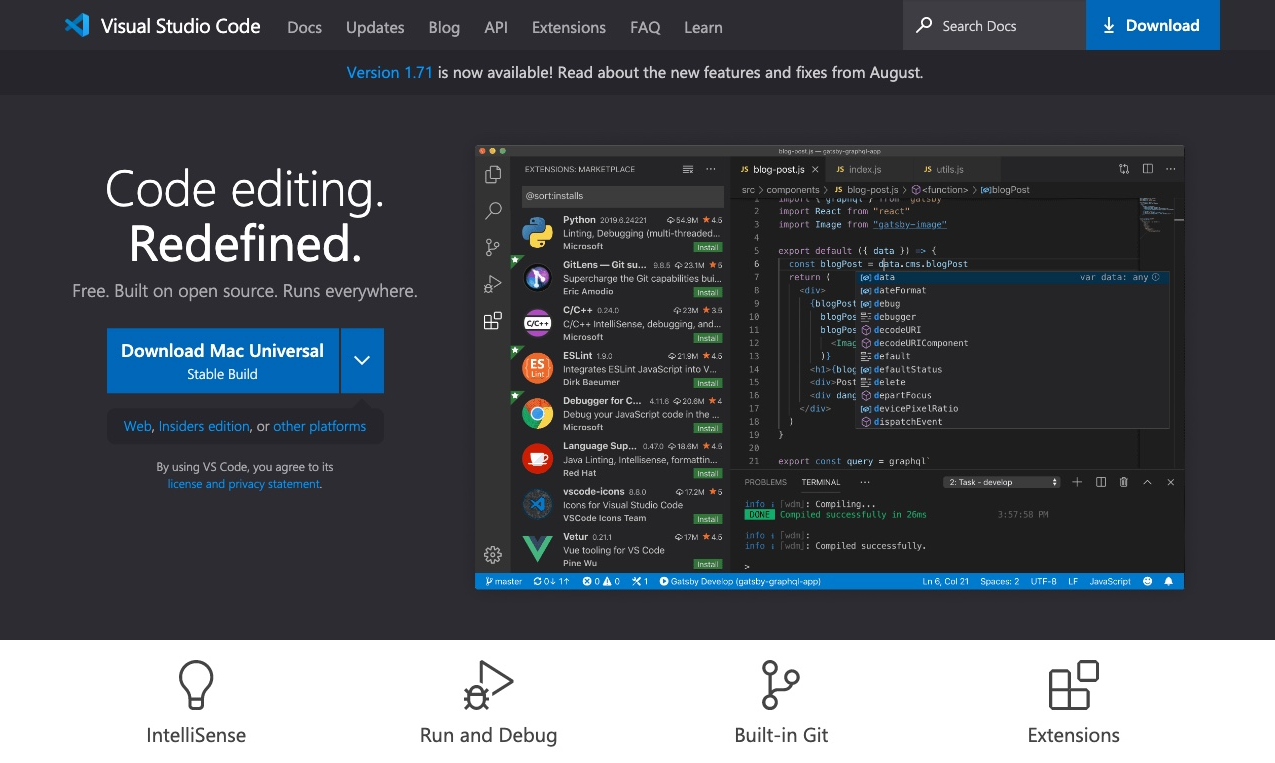
\includegraphics[width=0.7\linewidth]{./fig/appendix/vscode_install.png}
	\caption{VSCodeのインストール画面}
	\label{fig:vscode_install}
\end{figure}
脚注のURLで検索すると、インストール画面が出てきます。図~\ref{fig:vscode_install}がその画面です。どういう仕組みなのかはわからないのですが、自分のPC環境にあったVSCodeのバージョンが「Code editing. Redefined.」の下に出ているはずです。私の環境はintelチップのMacなのでこの表示になっていますが、自分のPC環境に本当に合っているのかどうか確かめてからインストールしましょう。Macではない場合は異なる表示になっていると思います。\par
ダウンロードが終わるとダウンロードフォルダに\texttt{VSCode-darwin-universal.zip}みたいなzipファイルがあるはずです。これをクリックするとVSCodeというアプリケーションが解凍されます。これをアプリケーションフォルダに移動すれば、インストール完了です。

\subsection{各種設定}
次に、使用に便利な一般の拡張機能を入れてみましょう。ブラウザで「VSCode 拡張機能 おすすめ」とか調べるととても参考になる記事が多いですが、そんな中から筆者が実際に使っているものをピックアップしていくつか紹介します。

\subsubsection{vscode-icons}
vscode-iconsはVSCodeで表示されるファイル類のアイコンをおしゃれにしてくれる機能です。アイコンがあると作業の際に視覚的にファイルを区別できて便利だと思います。

\subsubsection{indent-rainbow}
indent-rainbowはコード内のインデントを色分けして表示してくれる機能です。コーディングの際にはインデントを使って視認性を高くすることが重要です。また、Pythonではインデントがあることが\texttt{for}文や\texttt{if}文などで重要となります。そのインデントのレベルをわかりやすくしてくれます。

\subsubsection{Code Spell Checker}
Code Spell Checkerは、コードのスペルミスを指摘してくれる機能です。若干曲者で、Pythonの正しいコマンド名なのにスペルミスを指摘されることがあったり、固有名詞に対してスペルミスを指摘してきたりしますが、ユーザー辞書みたいなのに追加すれば対処できます。コードエラーの原因は些細なスペルミスだったりするので、便利な機能です。

\subsubsection{Error Lens}
Error Lensは警告などをわかりやすく表示してくれる機能です。
\begin{figure}
	\centering
	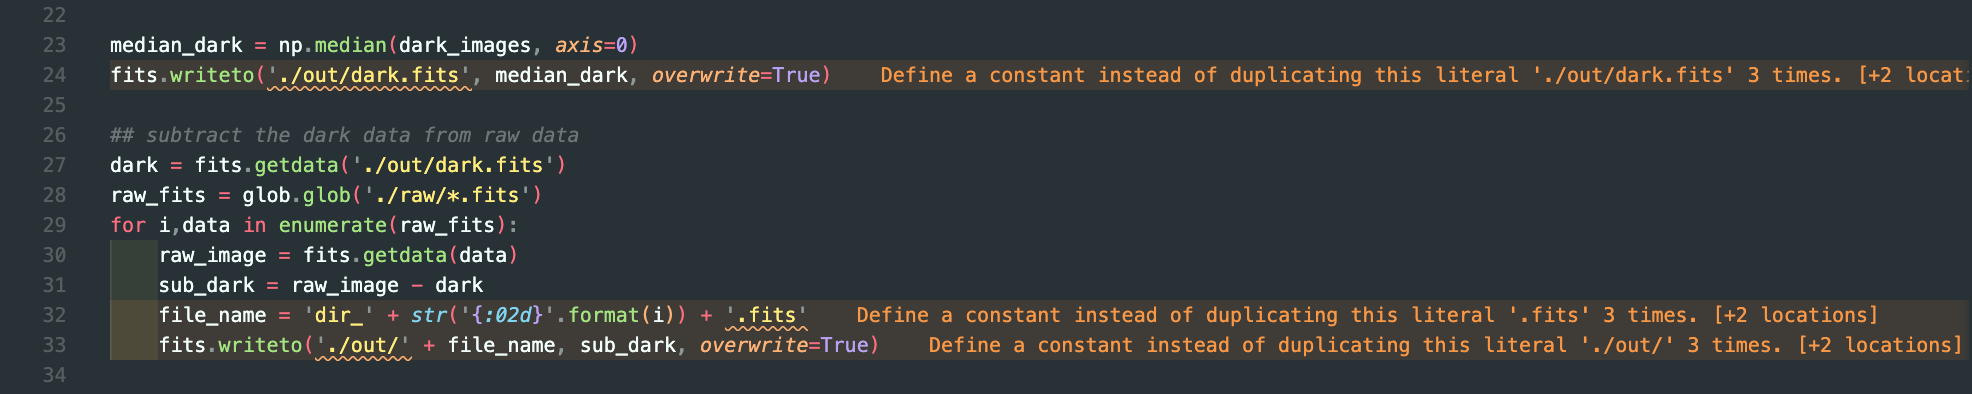
\includegraphics[width=0.8\linewidth]{./fig/appendix/error_lens.png}
	\caption{Error Lensによって表示された警告メッセージ}
	\label{fig:error_lens}
\end{figure}
例えば図~\ref{fig:error_lens}のような感じで警告を表示してくれます。

\subsubsection{Path Intellisense}
Path Intellisenseはディレクトリ名の補完をしてくれます。Pythonに限らず、コード内で相対的にディレクトリ指定を行うことは非常に多いので

\subsubsection{Prettier}
Prettier

\subsubsection{SonarLint}
SonarLint

\section{Python実行環境の構築}

\section{IRAF実行環境の構築}

\section{バグ取りの翁}

\section{Makali'i実習}

\section{SAOImage DS9実習}